\subsection{Mechanika zachowań klas jednostek}
\subsubsection{Jednostki walczące w zwarciu}
Zachowanie jednostek bliskiego zasięgu polega na wybraniu przeciwnika będącego w czerwonym obszarze (rys. \ref{fig:regions}), który ma najwyższą
wartość priorytetu obliczonego między innymi na podstawie odległości, ilości innych atakujących przeciwników oraz klasy celu.
Jednostka posiadająca cel ataku zmierza w jego kierunku, obierając najkrótszą drogę. Po dotarciu do celu podróży jednostki biorące udział w walce
losują naprzemiennie liczby, od których zależy wynik walki, jak i aktualnie wykorzystywana animacja.

\subsubsection{Jednostki walczące na dystans}
Takie jednostki wystrzeliwują w stronę przeciwników pociski, których celność jest reprezentowana przez dwie strefy (rys. \ref{fig:acc2}). Jedną oznaczającą 50\% celności,
czyli rozrzut, który będzie posiadała połowa pocisków, oraz drugą oznaczającą maksymalny rozrzut. Ten mechanizm pozwala na łatwe zamodelowanie
celności ze względu na odległość, wielkość celu oraz na osłony, za którymi może stać wroga jednostka.
\begin{figure}[h]
\centering
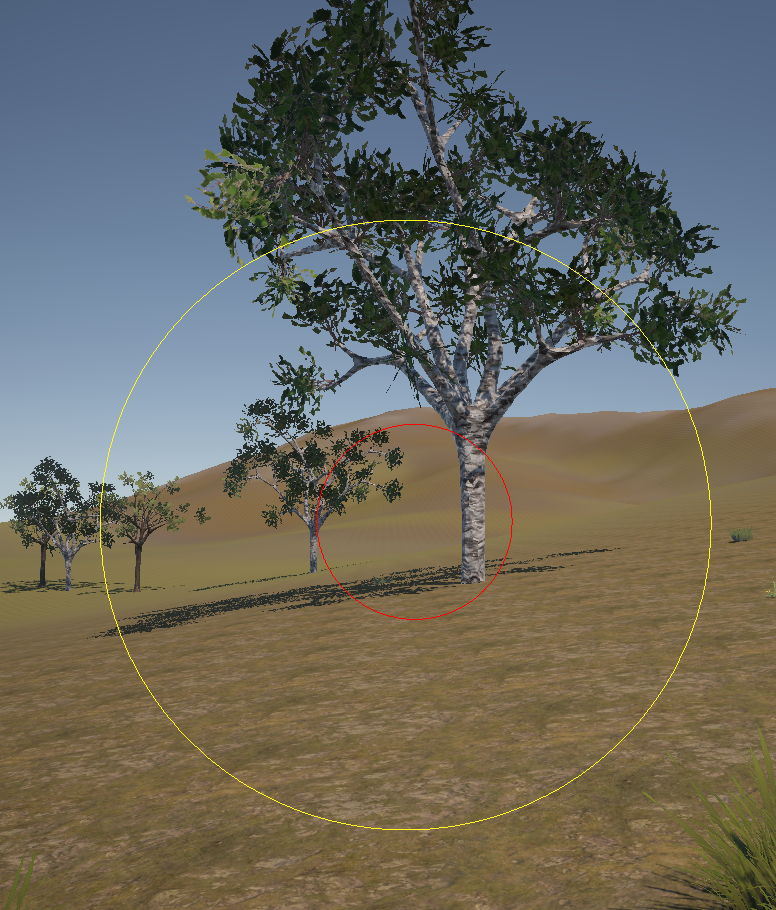
\includegraphics[width=0.6\textwidth]{images/acc}
\caption{Reprezentacja graficzna celowania widziana z perspektywy jednostki dalekozasięgowej. Czerwony okrąg reprezentuje obszar, w którym znajdzie się 50\% pocisków. Żółty obszar pokazuje maksymalny rozrzut.}
\label{fig:acc2}
\end{figure}
\subsubsection{Jednostki hybrydowe}
Obejmują zachowanie dwóch powyższych klas jednostek w zależności od odległości od przeciwnika.
W sytuacji, w której wroga jednostka znajduje się w pobliskim otoczeniu, wykorzystywany jest kod przeznaczony dla jednostek bliskiego zasięgu,
w przeciwnym przypadku wybierana jest logika jednostek zasięgowych.
